\documentclass[UTF8,a4paper,11pt,fontset=fandol]{ctexart}

\usepackage[a4paper,margin=2.3cm]{geometry}
\usepackage{graphicx}
\usepackage{hyperref}
\usepackage{enumitem}

\title{“网页空间布局”教学网站}
\author{可视化导论第一次作业}
\date{2026年9月17日}

\setlist[itemize]{leftmargin=2em,itemsep=2pt,topsep=3pt}
\hypersetup{colorlinks=true,linkcolor=blue,urlcolor=blue}

\begin{document}

\maketitle

\section{作品概述}

本站是一个面向《可视化导论》课程的中英双语教学网站，当前完成第一次作业“网页空间布局”。它并不罗列 CSS 属性，而是围绕“可视化课程作品浏览页”这一条案例，按“讲解、关键代码、展示”三个部分组织内容，帮助读者理解页面布局背后的空间关系与设计决策。

网站链接：\url{https://vis.starlab.top}

\section{关键亮点}

\subsection{统一的课程站点结构}

首页、关于页与各次作业页共用同一套导航、字体、颜色和间距。首页把作业组织成连续的课程目录，六条作业使用同一种卡片结构：已添加的 HW01 标记为“可查看”，其余标记为“未添加”且不设入口，读者据此一眼看出当前进度（图~\ref{fig:home-light}）。

后续新增作业只需补充对应章节，不必重新设计整站；未添加的作业已经预留占位页面，仍可从页头导航进入。整个项目因此具有连续性和扩展性。

\begin{figure}[htbp]
  \centering
  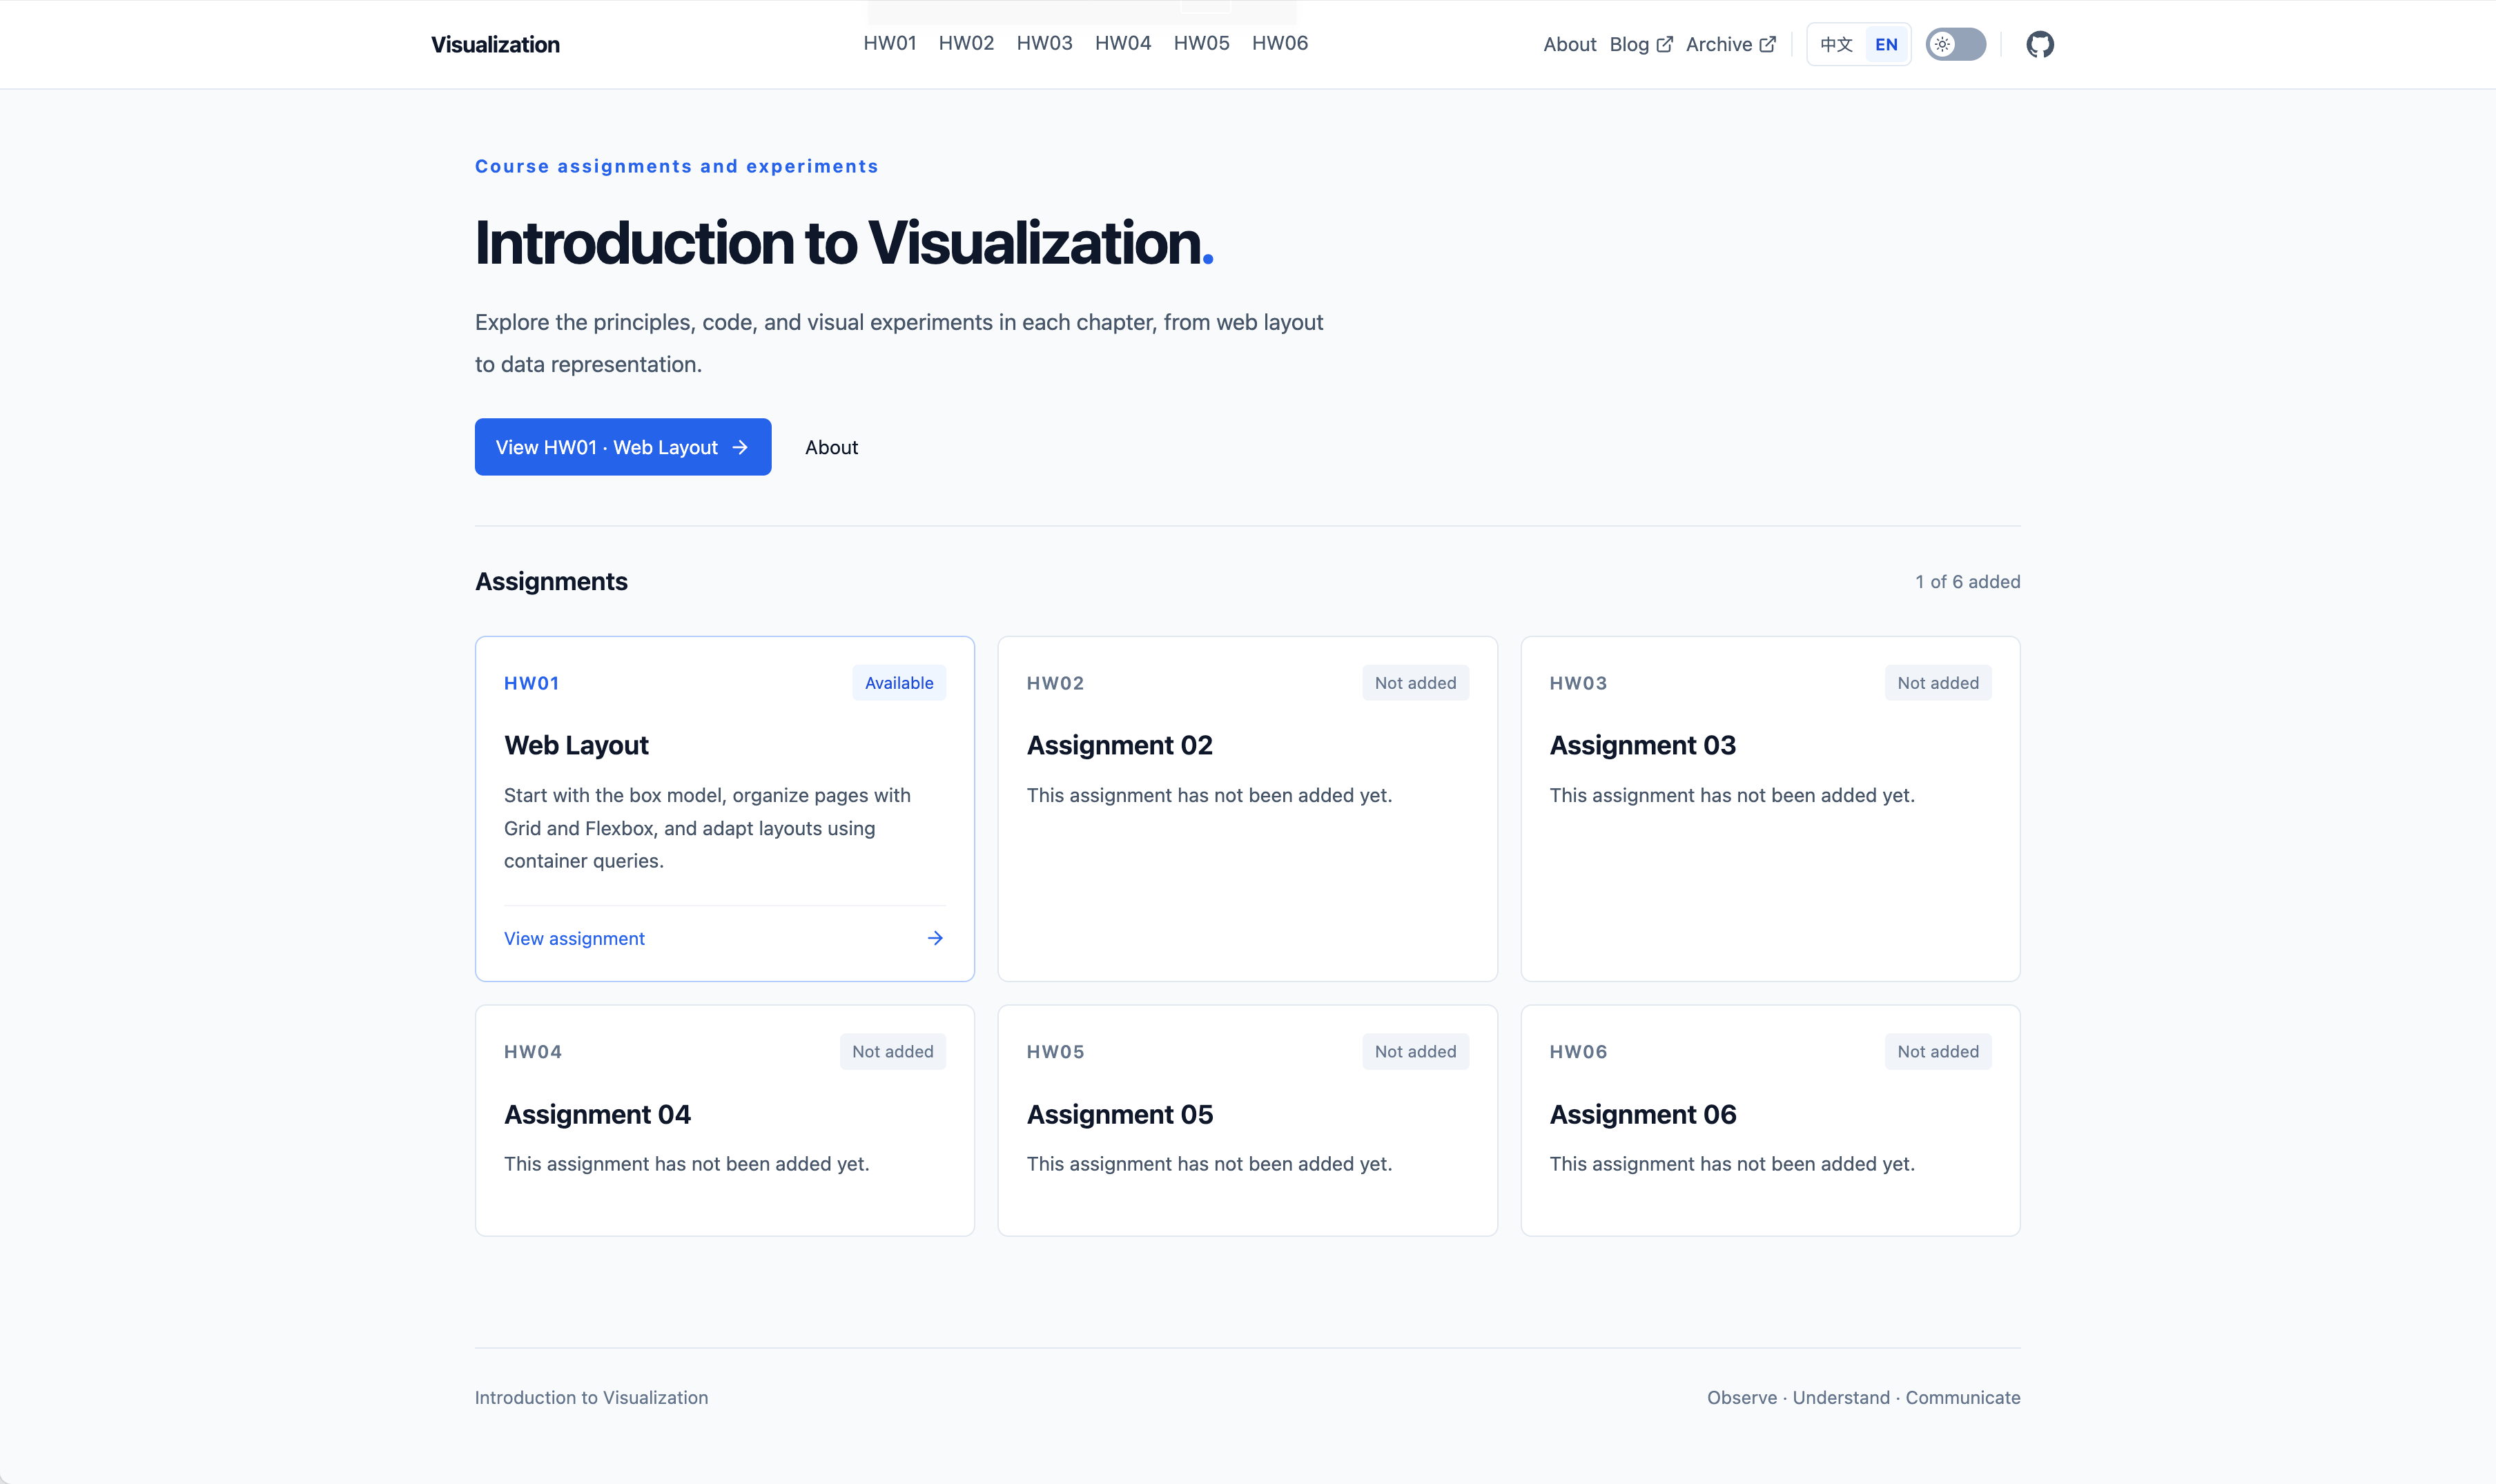
\includegraphics[width=0.96\textwidth]{screenshots/home-light.png}
  \caption{首页的作业目录与状态标记}
  \label{fig:home-light}
\end{figure}

\subsection{以案例贯穿的教学内容}

HW01 用同一条“可视化课程作品浏览页”案例逐步展开，六个步骤依次是：确定作品卡片的盒模型，让卡片内容保持正常流并处理局部定位，用 Grid 搭出作品浏览页骨架，用 Flex 排列作品工具栏，让作品页适应嵌入容器，最后验收完整案例。每一步都配有“讲解 / 关键代码 / 展示”三个标签（图~\ref{fig:hw01-chinese}）：讲解说明该步骤要解决的空间问题，关键代码给出对应的 HTML 与 CSS，展示把结果呈现出来。

图~\ref{fig:layout-explanation} 与图~\ref{fig:layout-code} 是同一步骤的两个侧面：讲解侧重设计理由，例如为什么这一行适合用 Flex 而不是 Grid；关键代码则给出可直接对照的实现。这样的组织方式强调的是布局的空间关系、信息层级与响应式适应，而不是单纯记忆语法。

\begin{figure}[htbp]
  \centering
  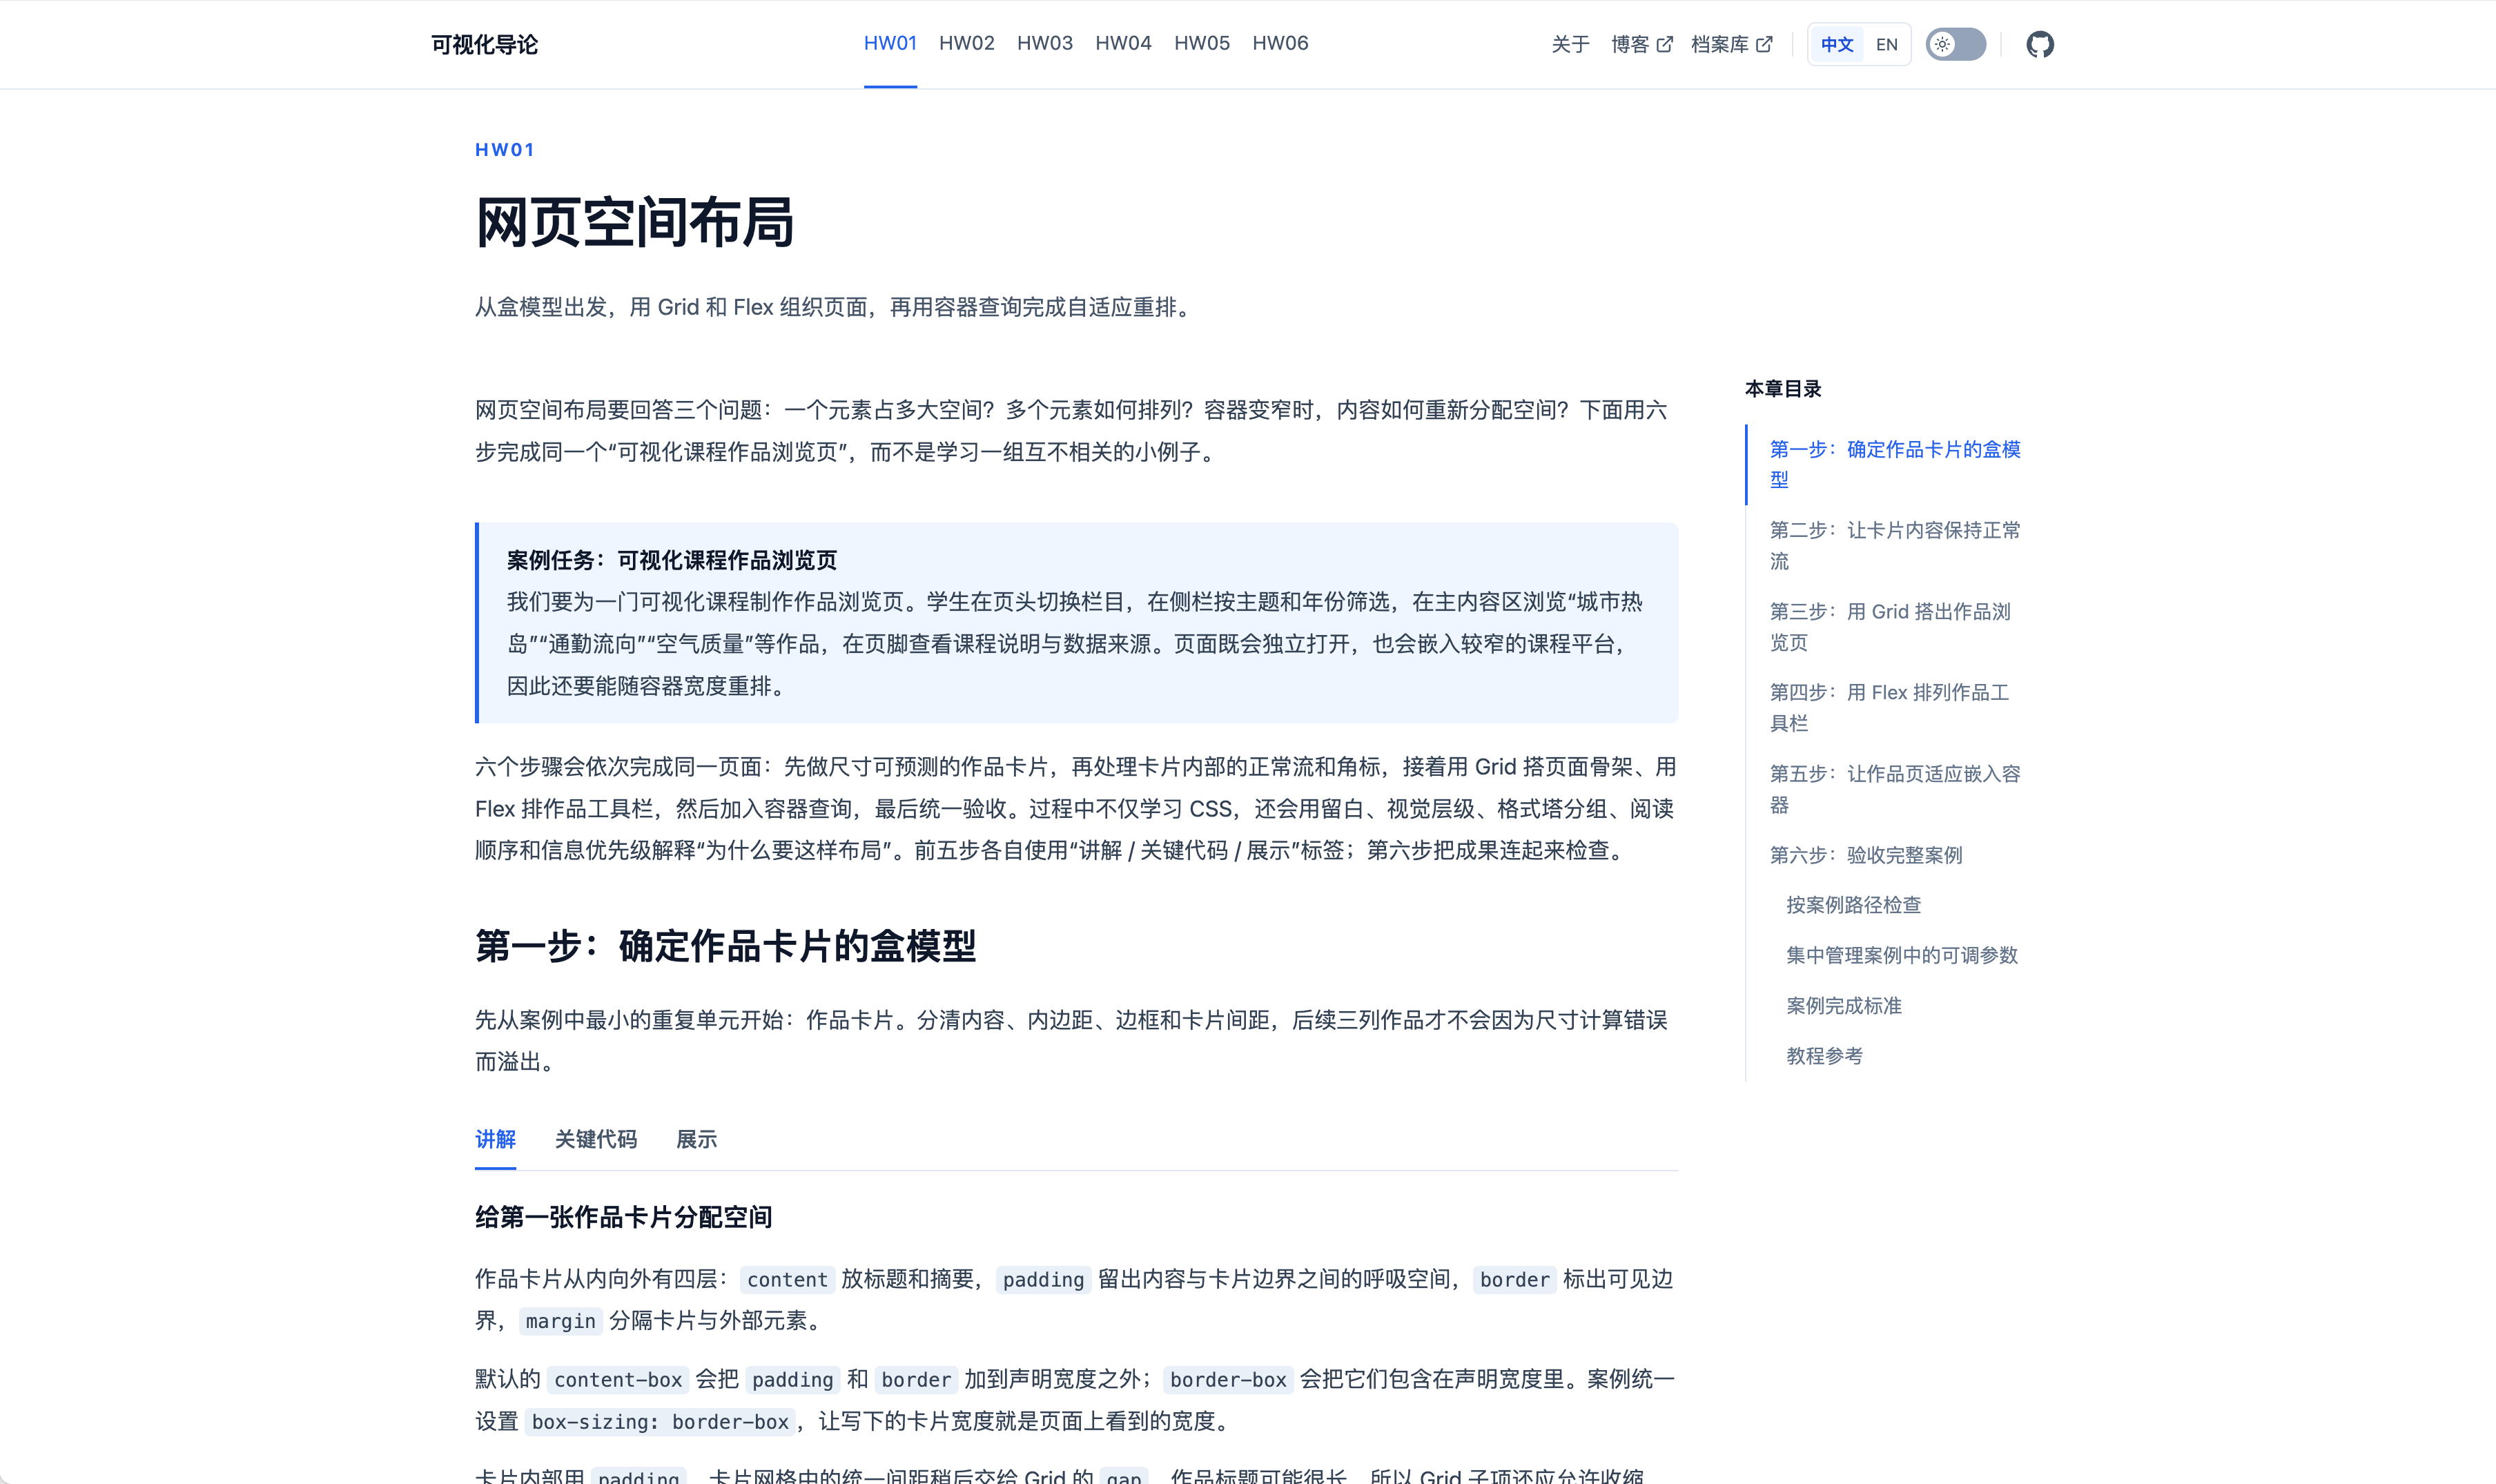
\includegraphics[width=0.96\textwidth]{screenshots/hw01-chinese.png}
  \caption{中文版 HW01 的“讲解 / 关键代码 / 展示”标签结构}
  \label{fig:hw01-chinese}
\end{figure}

\begin{figure}[htbp]
  \centering
  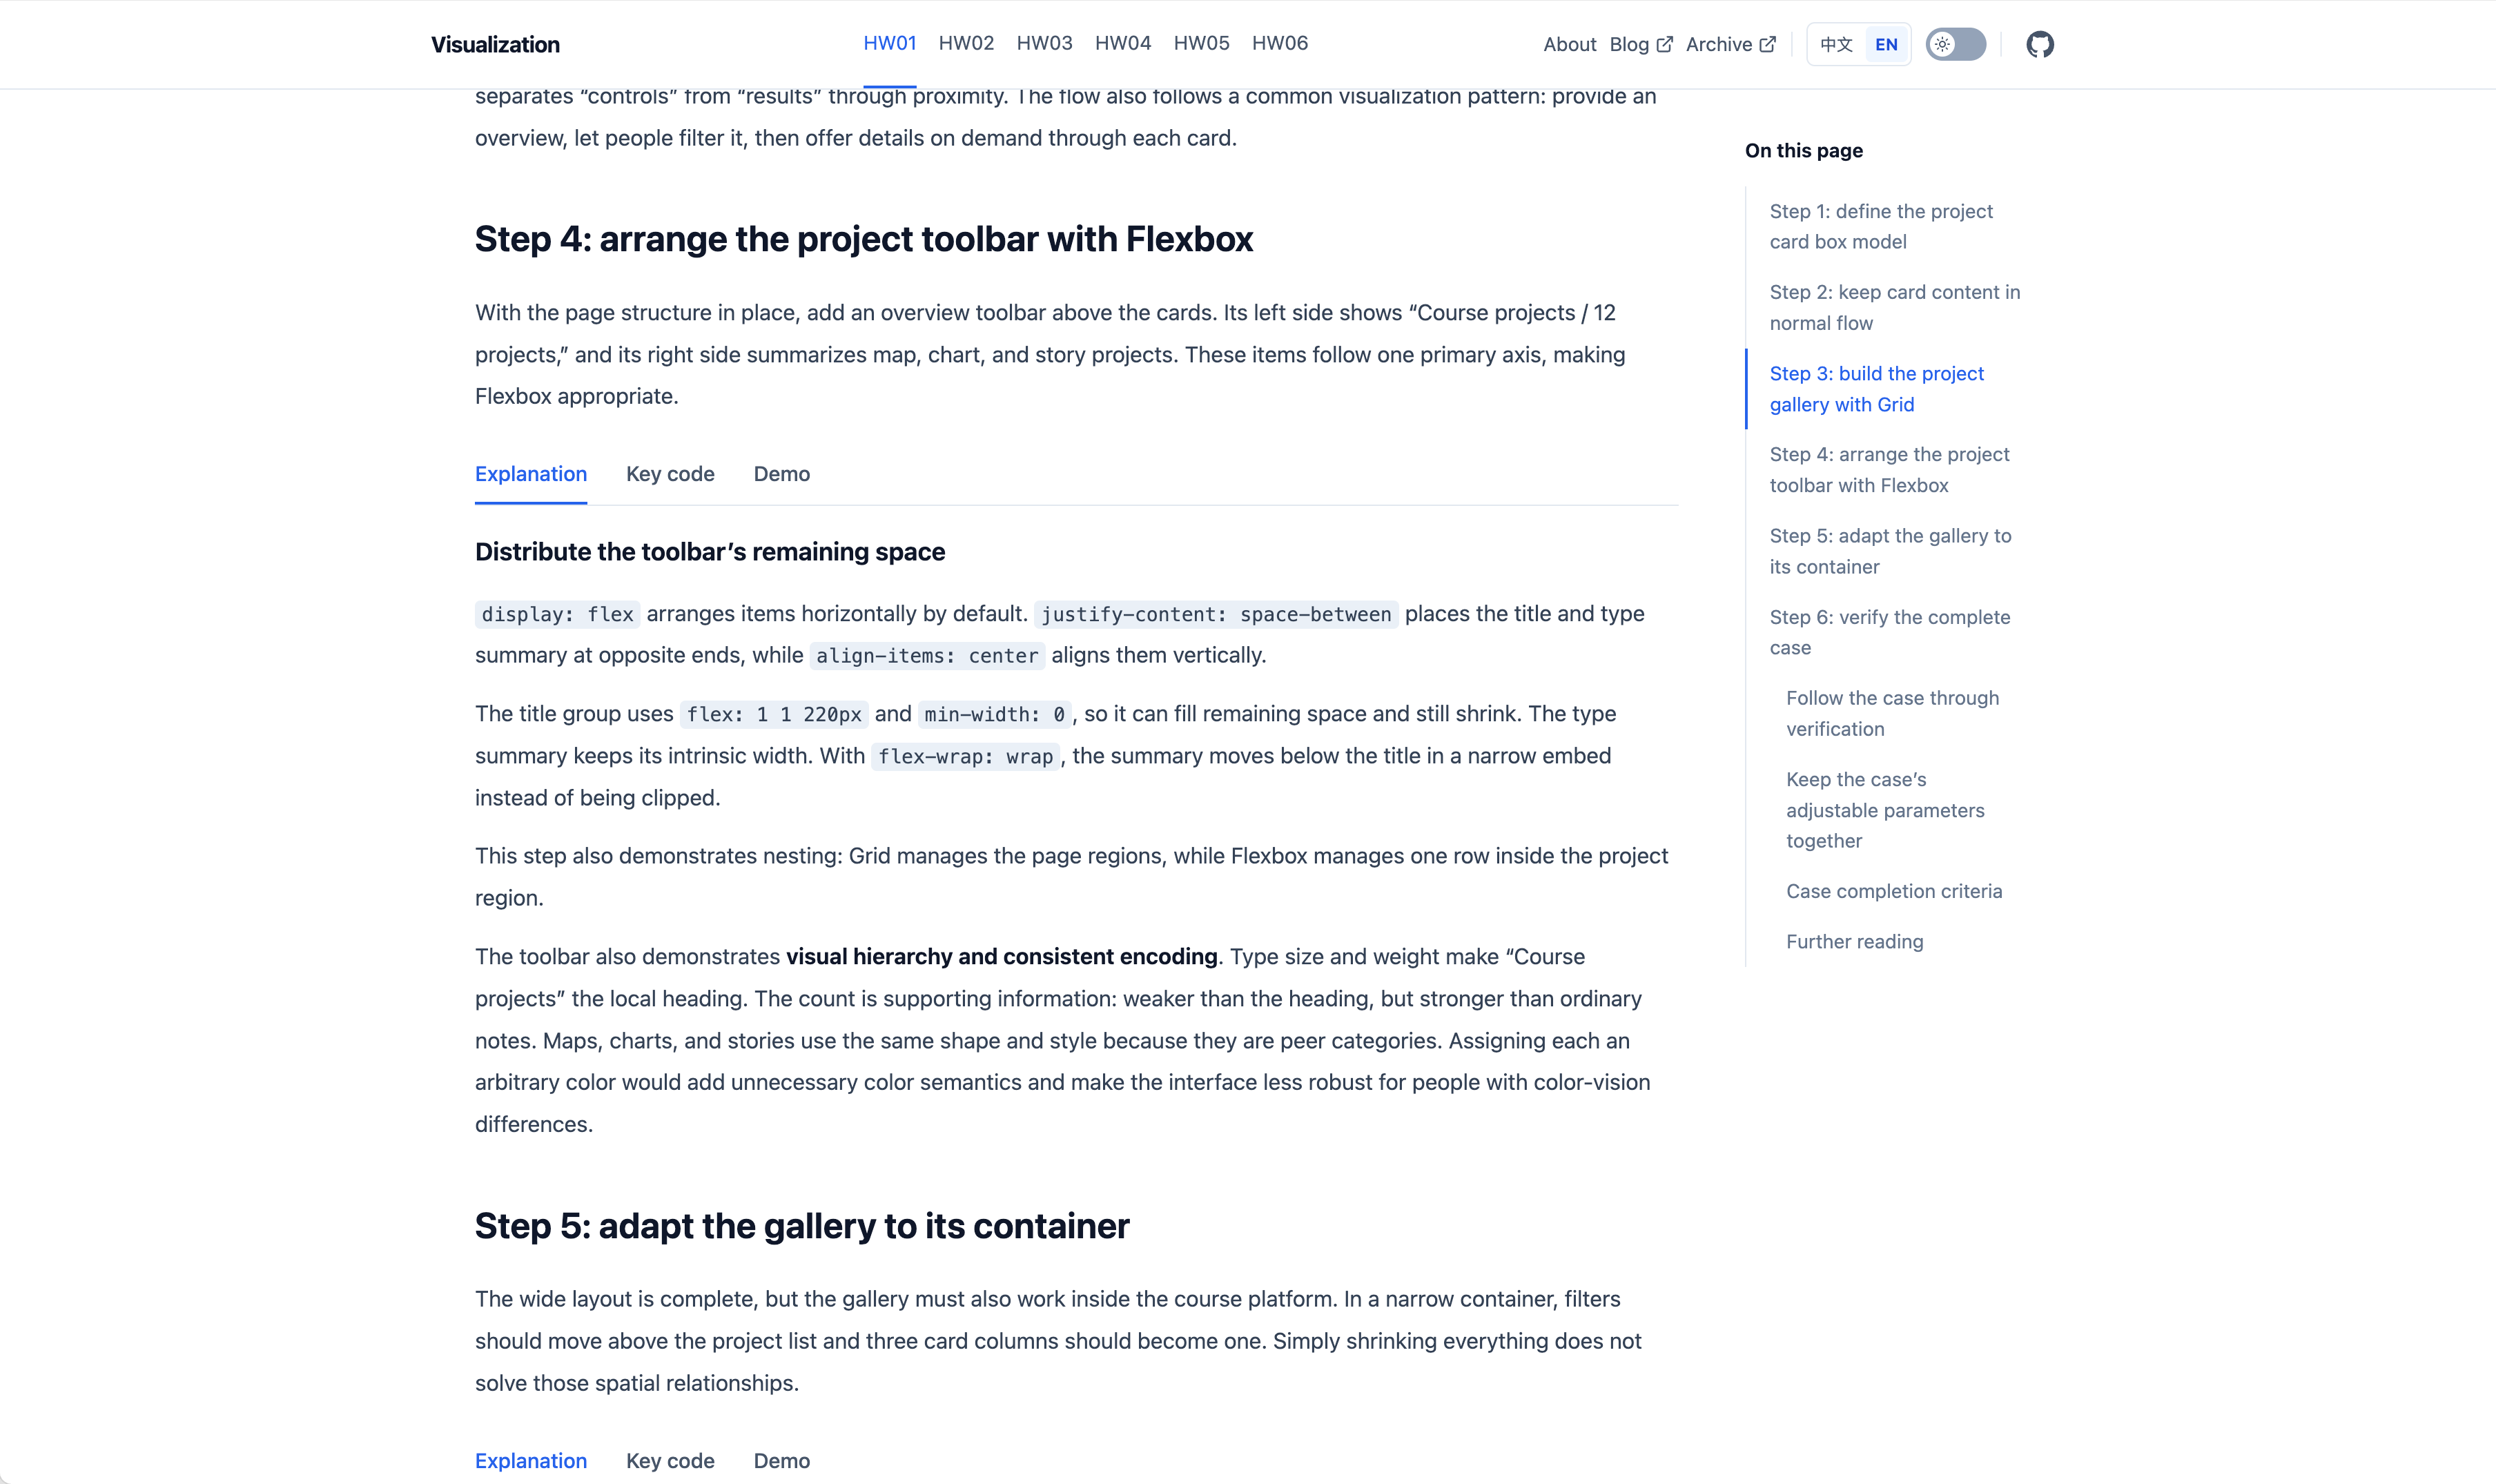
\includegraphics[width=0.96\textwidth]{screenshots/layout-explanation.png}
  \caption{英文版第四步的“讲解”标签}
  \label{fig:layout-explanation}
\end{figure}

\begin{figure}[htbp]
  \centering
  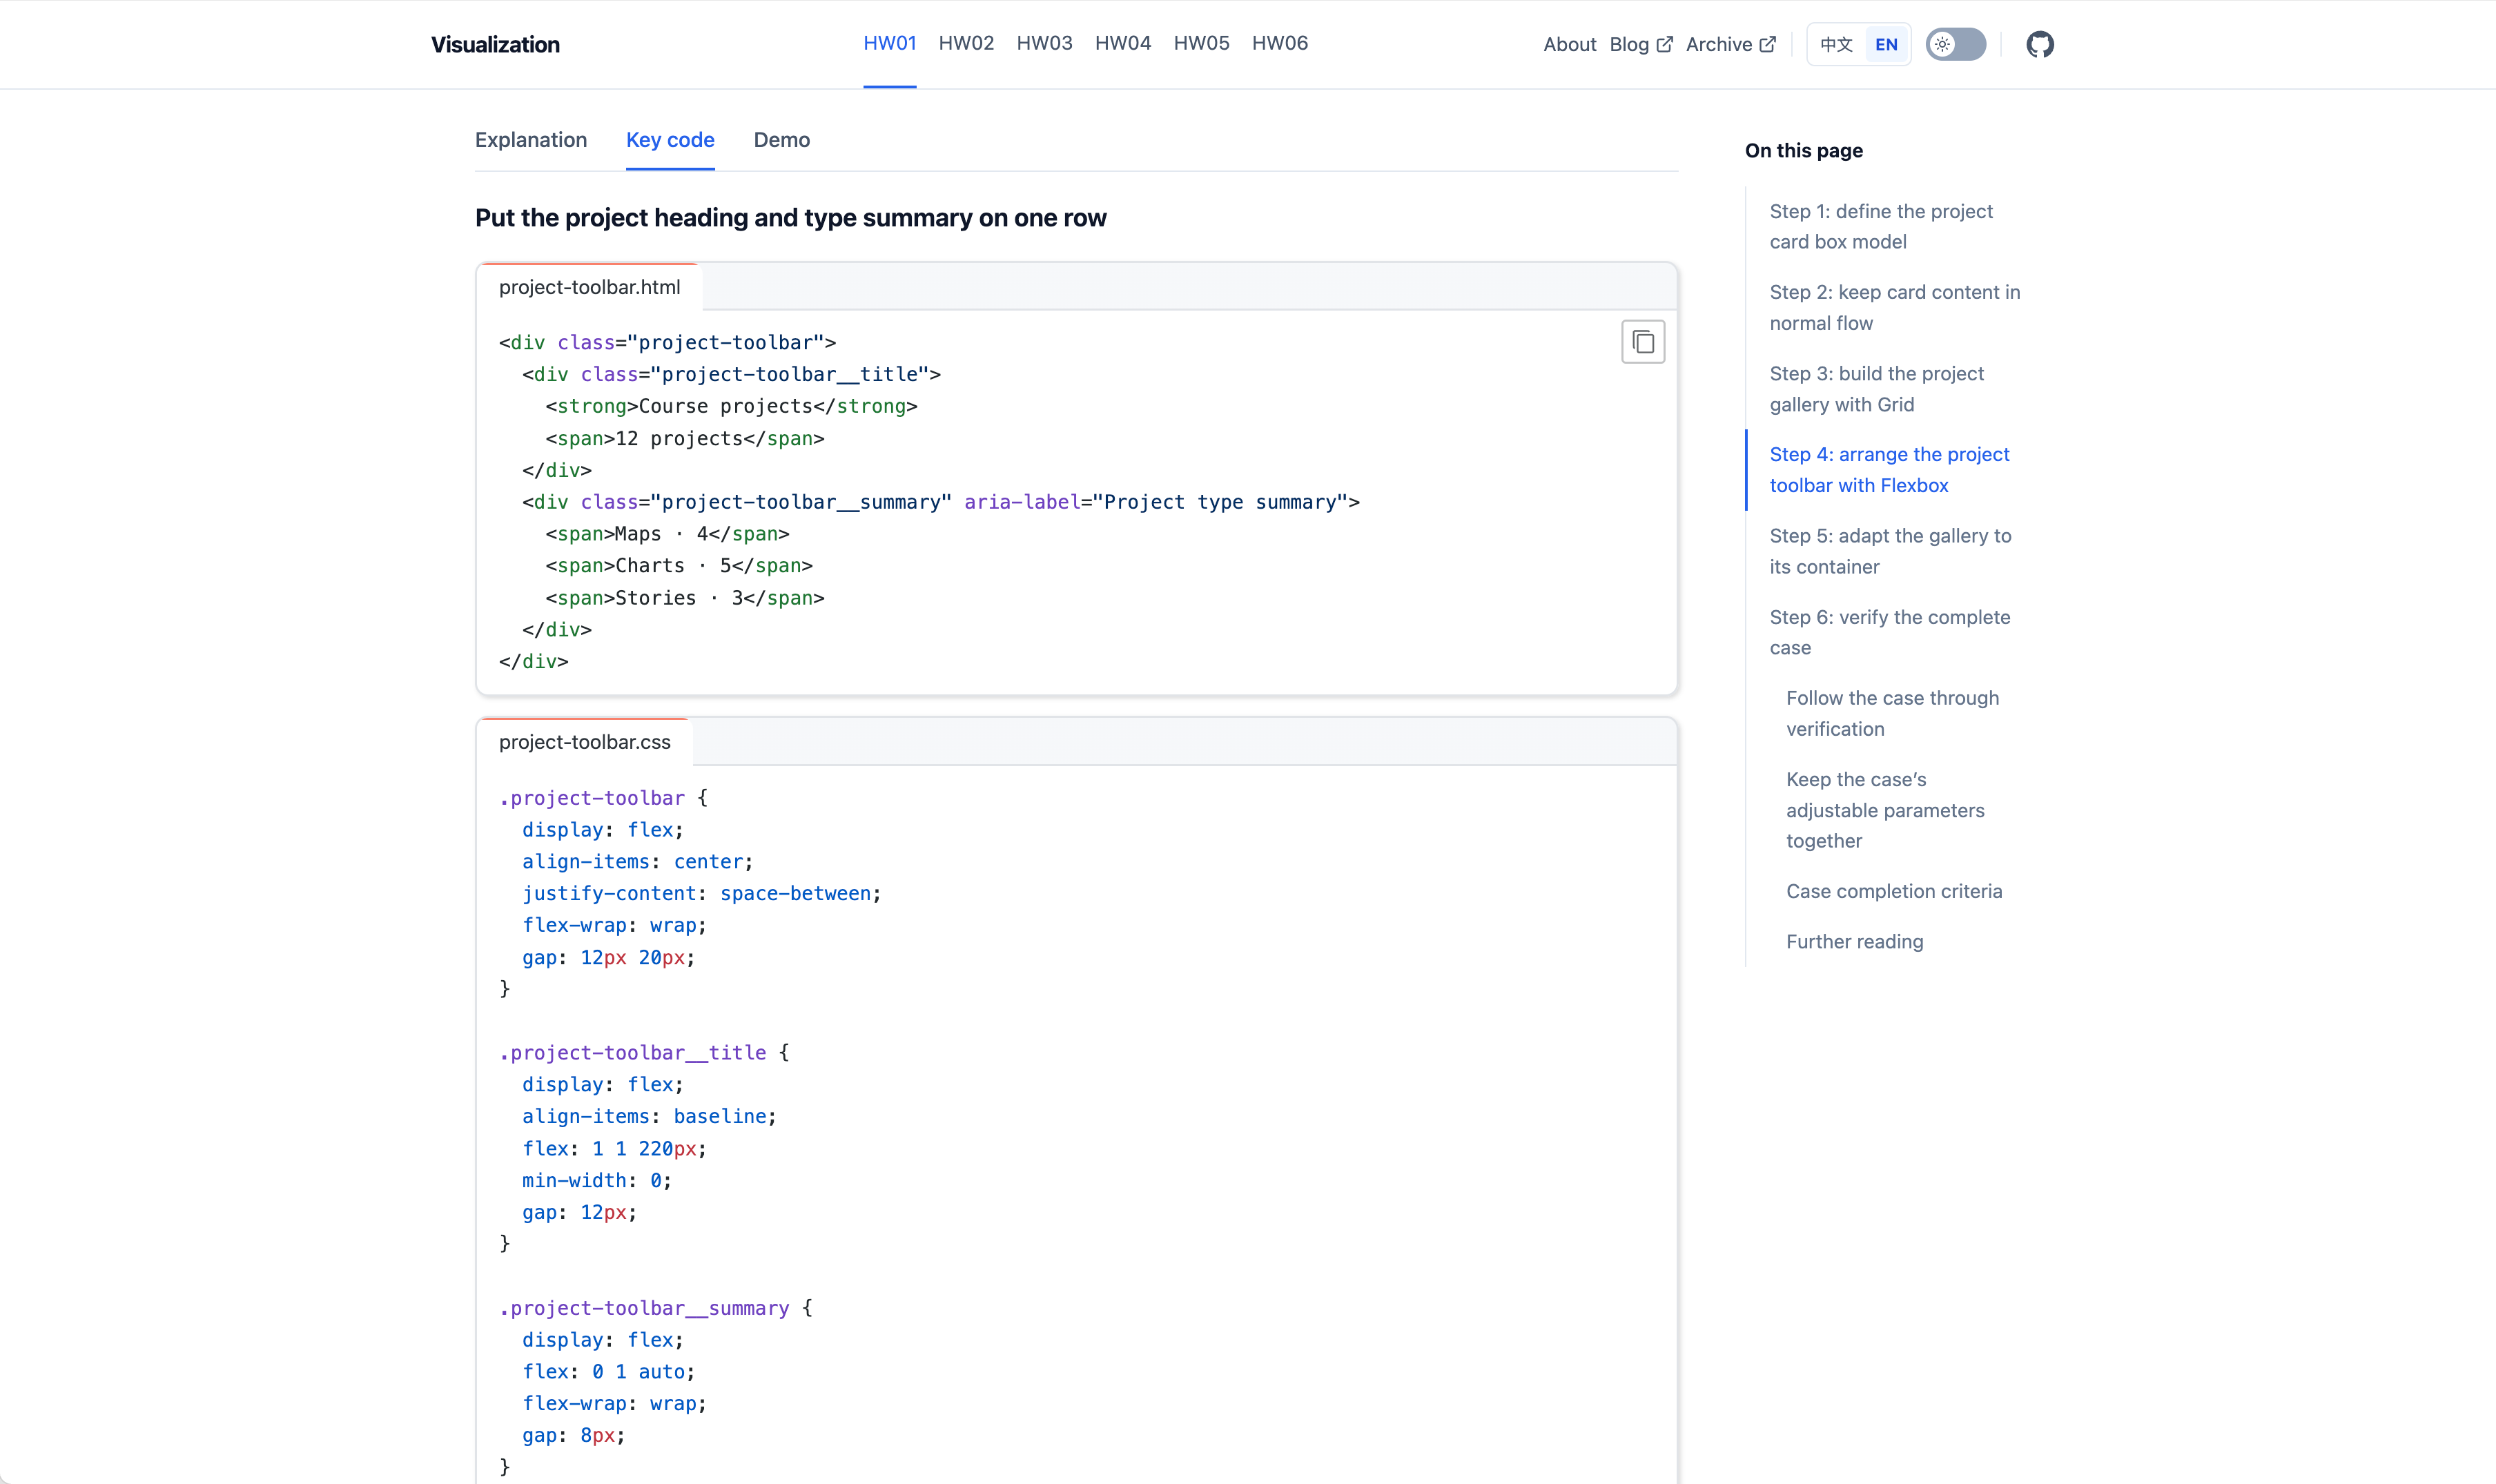
\includegraphics[width=0.96\textwidth]{screenshots/layout-code.png}
  \caption{英文版第四步的“关键代码”标签，右侧为本章目录}
  \label{fig:layout-code}
\end{figure}

\subsection{可操作的布局演示与响应式设计}

演示部分的交互程度并不相同。盒模型、正常文档流与 Grid 三步给出的是静态示意图，分别说明四层包含关系、定位前后的位置差异和区域映射，图内标注“非等比例”，以免读者误读尺寸。Flex 与布局实验台则可以操作：前者用“自适应宽度”和“窄容器”两个按钮切换预览宽度，观察工具栏在同一行与换行之间的变化；后者提供侧栏宽度、区域间距、区域内边距三个滑杆以及“恢复默认”，参数一经调整，布局立即响应。

响应式效果由容器查询完成。布局实验台在预览区域声明 \texttt{container-type: inline-size}，再用 \texttt{@container (max-width: 560px)} 判断自身可用宽度：把预览宽度设为“窄容器”后，不必改变浏览器窗口，页面即重排为单列，筛选区移到作品列表上方（图~\ref{fig:layout-demo}）。这与页面级媒体查询的差别，正是本步骤要说明的重点。

\begin{figure}[htbp]
  \centering
  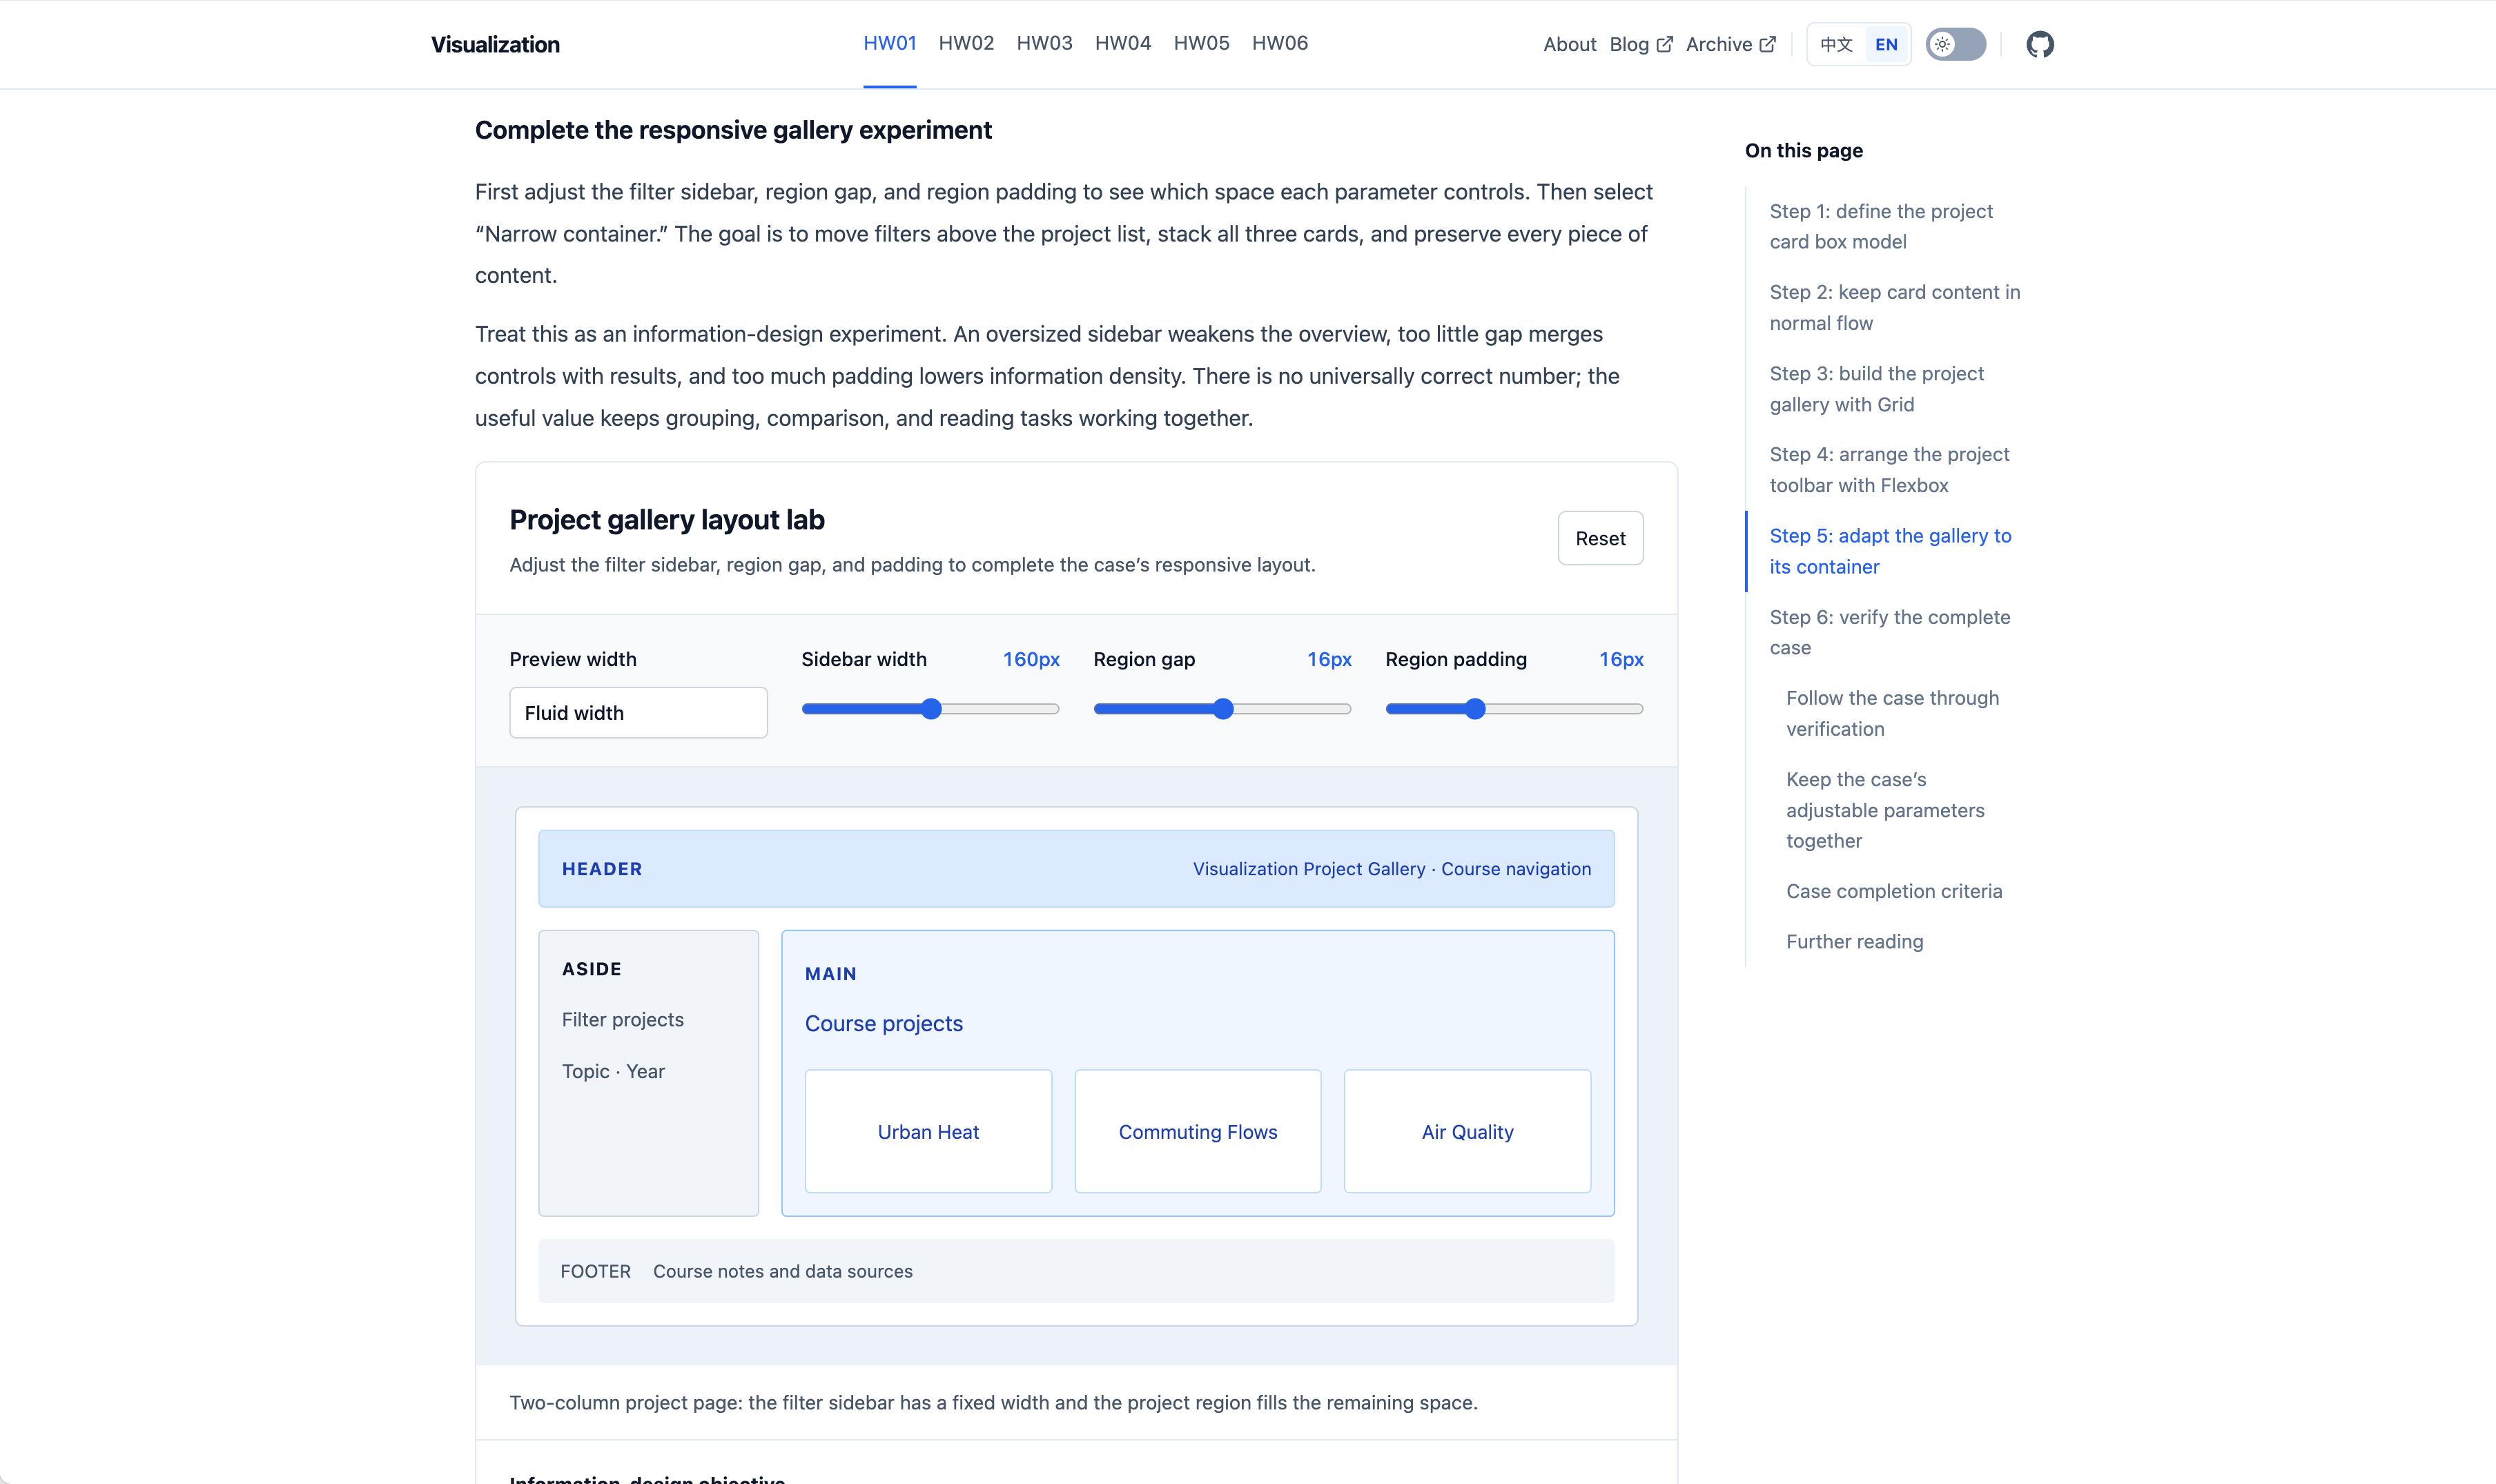
\includegraphics[width=0.96\textwidth]{screenshots/layout-demo.png}
  \caption{布局实验台的参数控件与窄容器下的重排}
  \label{fig:layout-demo}
\end{figure}

\subsection{阅读体验：无刷新双语切换、深色模式与本章目录}

中文与英文版本保持相同的章节顺序、教学内容和交互功能，分别位于 \texttt{/} 与 \texttt{/en/} 两套路由下。点击页头的语言入口时，页面只取回对应语言的内容并替换页头、正文和页脚，不进行整页刷新，因此滚动位置、当前标签页、演示参数、查询参数与锚点以及深色模式状态都得以保留，浏览器前进后退同样可用。若禁用 JavaScript，入口退化为普通链接，跳转仍然正常。

页头的另一侧是深色模式开关，状态保存在 \texttt{localStorage} 中；未作选择时跟随系统偏好，并在多个标签页之间同步（图~\ref{fig:home-dark}）。正文右侧是本章目录，由自定义 Remark 插件在构建时提取章节的二级和三级标题生成，标签页内部的标题不纳入其中；阅读滚动时目录会高亮当前所在的小节，视口窄于 1024px 时则收起为可展开的折叠项。

\begin{figure}[htbp]
  \centering
  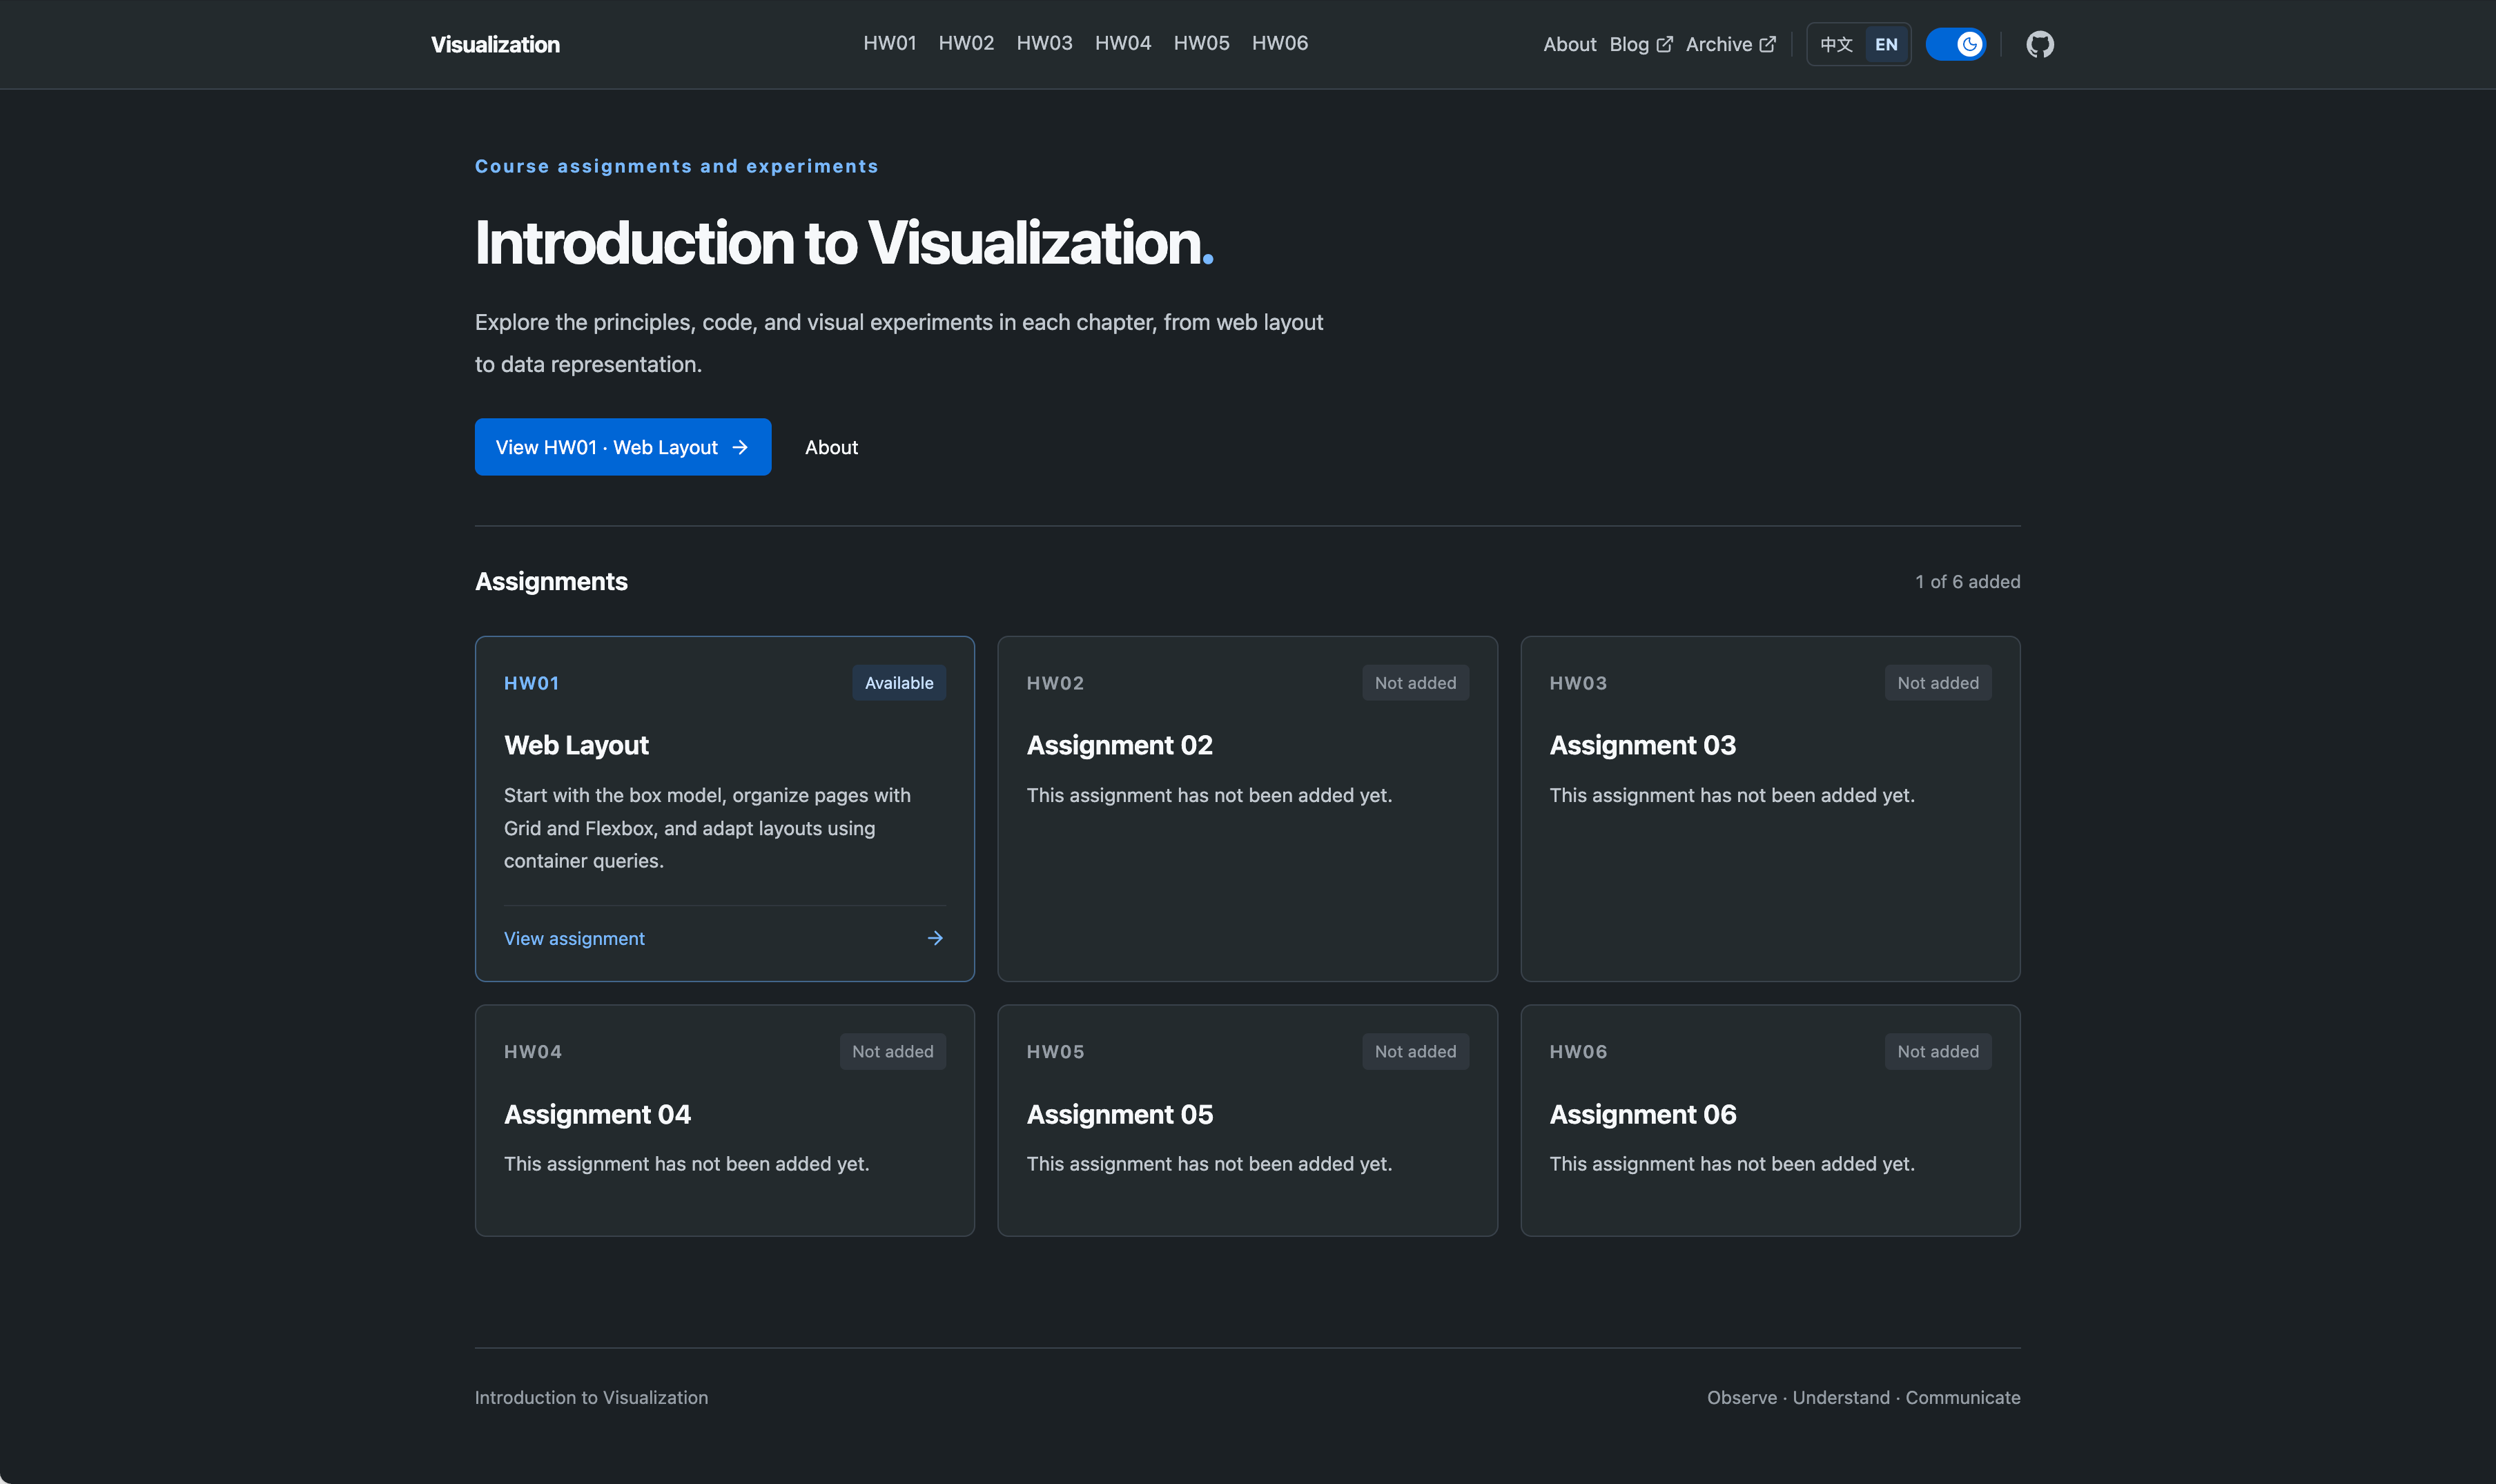
\includegraphics[width=0.96\textwidth]{screenshots/home-dark.png}
  \caption{英文首页、语言切换与深色模式控件}
  \label{fig:home-dark}
\end{figure}

\subsection{静态优先与构建验证}

建站采用静态优先架构，产物是可直接托管的 HTML、CSS 与 JavaScript，不依赖运行中的后端服务。基础页面无需 JavaScript 即可阅读，脚本只用于增强双语切换、标签页和布局实验等交互，因而适合部署到静态托管平台；当前线上环境部署于腾讯云 EdgeOne Makers。

构建完成后还可以再运行一组检查，读取 \texttt{dist/} 目录下的产物，核对中文与英文路由是否成对、语言属性与跨语言链接是否正确、站内链接是否都能落到实际文件、英文页面是否残留中文字符，以及各步骤的章节编号对应关系和五个演示组件、标签结构是否完整生成。

\section{设计思路总结}

本次作业希望表达的核心观点是：布局应当服务于内容关系与信息层级。正常文档流适合建立基础结构，Flex 适合一维排列，Grid 适合二维区域组织，容器查询则让组件依据自身实际可用空间调整，而不必依赖整个视口。把这些概念放进一条连续的案例，再配上可直接操作的参数与即时的视觉反馈，理论、代码与视觉效果就不再是彼此分离的三件事。

\end{document}
